% ****** Start of file apssamp.tex ******
%
%   This file is part of the APS files in the REVTeX 4.2 distribution.
%   Version 4.2a of REVTeX, December 2014
%
%   Copyright (c) 2014 The American Physical Society.
%
%   See the REVTeX 4 README file for restrictions and more information.
%
% TeX'ing this file requires that you have AMS-LaTeX 2.0 installed
% as well as the rest of the prerequisites for REVTeX 4.2
%
% See the REVTeX 4 README file
% It also requires running BibTeX. The commands are as follows:
%
%  1)  latex apssamp.tex
%  2)  bibtex apssamp
%  3)  latex apssamp.tex
%  4)  latex apssamp.tex
%
\documentclass[%
 reprint,
%superscriptaddress,
%groupedaddress,
%unsortedaddress,
%runinaddress,
%frontmatterverbose, 
%preprint,
%preprintnumbers,
%nofootinbib,
%nobibnotes,
%bibnotes,
 amsmath,amssymb,
 aps,
%pra,
%prb,
%rmp,
%prstab,
%prstper,
%floatfix,
]{revtex4-2}

\usepackage{booktabs}
\usepackage{graphicx}% Include figure files
\usepackage{dcolumn}% Align table columns on decimal point
\usepackage{bm}% bold math
\usepackage{enumitem}
\usepackage[mathlines]{lineno}% Enable numbering of text and display math
%\linenumbers\relax % Commence numbering lines

%\usepackage[showframe,%Uncomment any one of the following lines to test 
%%scale=0.7, marginratio={1:1, 2:3}, ignoreall,% default settings
%%text={7in,10in},centering,
%%margin=1.5in,
%%total={6.5in,8.75in}, top=1.2in, left=0.9in, includefoot,
%%height=10in,a5paper,hmargin={3cm,0.8in},
%]{geometry}
\usepackage[english, spanish, mexico, es-noitemize]{babel}
\usepackage[pdfusetitle, colorlinks]{hyperref}
\hypersetup{
    colorlinks=true,    % Colores en lugar de cajas
    linkcolor=gray,
    citecolor=black, % Color de los enlaces internos
    filecolor=gray,  % Color de los enlaces a archivos
    urlcolor=gray       % Color de los enlaces externos
}
%\usepackage[shortlabels, inline]{enumitem}
\usepackage{array}
%\usepackage{titlesec}
%\usepackage[titles]{tocloft}
%\usepackage{xcolor, xpatch, calc}
%\usepackage{graphicx, booktabs}
%\usepackage{pgfplots}
%\usepackage[outline]{contour}
%\usepackage[hang, labelfont=bf, labelsep=period, margin=0.5in]{caption}
\usepackage{subcaption}
%\usepackage{csquotes}
\usepackage{lipsum}
%\usepackage{blindtext}
\usepackage{amsmath}
\usepackage{graphicx}
%\usepackage{svg}
%\usepackage{booktabs}
%\usepackage{enumitem}
\usepackage{float}
\usepackage{listings}
\usepackage{xcolor}
\usepackage{listings}
\lstset{
  language=Python,
  basicstyle=\ttfamily\small,
  commentstyle=\itshape\color{gray},
  keywordstyle=\bfseries\color{blue},
  numbers=left,
  numberstyle=\tiny\color{gray},
  stepnumber=1,
  numbersep=5pt,
  backgroundcolor=\color{white},
  frame=single,
  breaklines=true,
  breakatwhitespace=false,
  captionpos=b,
  tabsize=2,
  showspaces=false,
  showstringspaces=false
}

\usepackage{appendix}


\begin{document}

\preprint{APS/123-QED}

\title{Simulación de percolación en mallas bidimensionales cuadradas}% Force line breaks with \\

 
\author{M. Barrios}
\email{mibarriosg@unal.edu.co}
\author{J. Segura}
\email{jusegurag@unal.edu.co}
\author{A. Silva}
\email{ansilvav@unal.edu.co}
\affiliation{Introducción a la Computación Científica y de Alto Rendimiento [2015174]\\Universidad Nacional de Colombia\\ Departamento de Física - Bogotá D.C}%
\date{\today}% It is always \today, today,
             %  but any date may be explicitly specified
\begin{abstract}
\begin{description}
\item[Resumen] En este trabajo se estudió el fenómeno de percolación por sitio en mallas bidimensionales cuadradas mediante simulaciones computacionales en C++. El objetivo principal fue analizar, para distintos tamaños de malla y probabilidades de ocupación, la probabilidad de aparición de un cluster percolante, el tamaño promedio del cluster percolante más grande y el tiempo computacional requerido para su detección. Se implementó un algoritmo basado en búsqueda en profundidad, optimizado para detectar conectividad a partir de los bordes de la malla. Se ejecutaron simulaciones variando la dimension de la malla $L$, la probabilidad de ocupación $p$, y el nivel de optimización del compilador (desde \texttt{-O0} hasta \texttt{-Ofast}), con $50$ semillas diferentes para cada configuración de $L$, $p$ y nivel de optimización. Además, se automatizaron las tareas como la compilación, la ejecución, \textit{unit testing}, \textit{profiling}, \textit{debugging} y la generación de gráficos mediante un Makefile. Los procesos se ejecutaron en paralelo mediante \textit{GNU parallel}, permitiendo un mejor aprovechamiento de recursos. Los resultados muestran el comportamiento crítico esperado del sistema para la probabilidad de percolación, se observó convergencia en la proporción del tamaño del cluster percolante más grande respecto al tamaño de la malla para valores de probabilidad de ocupación mayores a la probabilidad de ocupación crítica $p_c$ y un aumento exponencial en los tiempos computacionales conforme la malla es más grande, al igual que mejoras sustanciales de rendimiento con los diferentes niveles de optimización del compilador.


\end{description}
\begin{description}
\item[Palabras clave] Percolación, cluster, tiempo computacional, optimización, \textit{profiling}, \textit{debugging}, \textit{unit testing}, probabilidad de ocupación crítica.

\end{description}
\end{abstract}

\maketitle

\section{Introducción}

El fenómeno de percolación es un modelo fundamental en física estadística y teoría de redes, con aplicaciones que abarcan desde la propagación de incendios forestales y epidemias hasta la conductividad de materiales porosos. En su forma más simple, el modelo de percolación representa un sistema en el cual cada sitio (o enlace) de una red es ocupado con cierta probabilidad $p$, y se estudia la formación de caminos conectados a través del sistema.

En este trabajo se considera el modelo de percolación por sitio en una malla bidimensional cuadrada de tamaño $L \times L$, donde cada celda se ocupa de forma independiente con probabilidad $p$. Dos celdas ocupadas se consideran conectadas si son vecinas en la dirección de von Neumann (norte, sur, este u oeste). A partir de estas conexiones se forman clusters o componentes conexas de celdas ocupadas.

Un aspecto central del modelo es la transición de fase que ocurre en el límite termodinámico ($L \to \infty$): existe un valor crítico de $p$, denotado $p_c$, por debajo del cual la probabilidad de que exista un cluster que atraviese el sistema es prácticamente nula, y por encima del cual la percolación ocurre casi con certeza. En este proyecto, se estudian tres aspectos fundamentales del comportamiento del sistema en función de $p$ y del tamaño $L$:

\begin{enumerate}
    \item La probabilidad de percolación, es decir la fracción de configuraciones en las que existe un cluster que conecta lados opuestos de la malla, ya sea en dirección vertical (de arriba a abajo) o horizontal (de izquierda a derecha).
    \item El tamaño promedio del cluster más grande para en función de la probabilidad $p$ para cada $L$.
    \item El efecto que tiene el nivel de optimización del compilador \texttt{-O} en el tiempo de computo en función del tamaño del sistema $L$.
\end{enumerate}

Dado el carácter probabilístico del modelo, las simulaciones se repiten 50 veces (50 \texttt{seed} diferentes) para cada valor de $p$, de $L$, y \texttt{-O} con el fin de obtener estimaciones precisas de las cantidades de interés. A partir de estas repeticiones se calculan promedios y desviaciones estándar, lo que permite evaluar la estabilidad y confiabilidad de los resultados.

Desde el punto de vista computacional, el código fue implementado en C++ siguiendo una estructura modular. Se utilizó un Makefile para automatizar tanto la ejecución del programa como el proceso de análisis del desempeño. Este análisis incluyó tareas como depuración, pruebas unitarias, medición de cobertura de código y perfilamiento, mediante \textit{targets} específicos, los cuales se describen en detalle en la sección de metodología.

\section{Metodología}

\subsection{Código base}

El programa se estructuró de manera modular en tres archivos principales:

\begin{itemize}
    \item \texttt{functions.h}: contiene las declaraciones de funciones y las inclusiones de librerías necesarias para el resto del programa.
    
    \item \texttt{functions.cpp}: implementa las funciones que permiten analizar la malla, entre ellas las funciones principales \texttt{hay\_cluster\_percolante()} y \texttt{dfs()}, encargadas de identificar y etiquetar los clusteres, así como de detectar si alguno de ellos es percolante. Estas funciones se describen con mayor detalle más adelante.
    
    \item \texttt{main.cpp}: actúa como punto de entrada del programa. Recibe por línea de comandos los parámetros \texttt{L} (dimensión de la malla), \texttt{p} (probabilidad de ocupación), \texttt{seed} (semilla aleatoria) y \texttt{bool\_grafica} (que si es 1 grafica la malla y si es 0 no). Con estos valores, genera una malla binaria aleatoria de tamaño representada en un vector unidimensional de tipo \texttt{bool} y longitud \texttt{LxL}. También inicializa un vector \texttt{etiquetas} con ceros, del mismo tamaño, para registrar la pertenencia de cada sitio a un cluster, una variable \texttt{tamano\_max} y un vector \texttt{percolantes} vacío que almacenará las etiquetas de los clusteres que percolan tras el llamado a la función \texttt{hay\_cluster\_percolante()}. Durante todo este proceso mide el tiempo de ejecución (tanto \textit{CPU time} como \textit{wall time}) e imprime finalmente por consola si hay percolación, el tamaño del cluster percolante más grande y los tiempos registrados.
    
\end{itemize}

Ahora, procedemos a explicar la lógica de las dos funciones principales en las que recae el programa:

La función \texttt{hay\_cluster\_percolante()} recibe como argumento el vector de la \texttt{malla}, el tamaño \texttt{L}, la variable \texttt{tamano\_max}, el vector \texttt{etiquetas} y el vector \texttt{percolantes}. Esta recorre los sitios ocupados de la primera fila y la primera columna de la malla de tamaño \texttt{LxL}. Si alguno de estos sitios aún no ha sido etiquetado (es decir, si su valor en el vector \texttt{etiquetas} es cero), se lanza una búsqueda en profundidad llamando a la función \texttt{dfs()}.

La función \texttt{dfs()} toma como entrada la posición inicial del sitio (\texttt{id}), el tamaño de la malla (\texttt{L}), una etiqueta entera única (\texttt{etiqueta}) para identificar el cluster actual, el vector binario de la malla (\texttt{malla}), un vector de etiquetas para marcar los sitios ya visitados (\texttt{etiquetas}), y cuatro referencias booleanas (\texttt{toca\_arriba}, \texttt{toca\_abajo}, \texttt{toca\_izquierda}, \texttt{toca\_derecha}) que se actualizan si el cluster llega a los bordes respectivos. La función \texttt{dfs()} explora todos los sitios conectados al sitio inicial (\texttt{id}) que están ocupados y aún no etiquetados, asignándoles la etiqueta correspondiente y devolviendo el tamaño total del cluster encontrado. 

De vuelta en \texttt{hay\_cluster\_percolante()}, si el cluster encontrado cumple la condición de tocar simultáneamente los bordes superior e inferior (\texttt{toca\_arriba \&\& toca\_abajo}) o izquierdo y derecho (\texttt{toca\_izquierda \&\& toca\_derecha}), se considera un cluster percolante. En tal caso, se actualiza la variable \texttt{tamano\_max} si el nuevo cluster es mayor a los previos, y se agrega su etiqueta al vector \texttt{percolantes}.

Opcionalmente, si al ejecutar la función se pasa por consola el valor \texttt{bool\_grafica = 1}, \texttt{main.cpp} puede llamar a la función \texttt{imprimir\_clusters()}, que exporta la malla etiquetada a un archivo \texttt{.txt}. En este archivo, los sitios no ocupados se marcan con \texttt{0}, los ocupados que no forman parte de clusteres percolantes con \texttt{1}, y los clusteres percolantes con etiquetas enteras crecientes a partir de \texttt{2}. Esta salida se utiliza para visualizar gráficamente los clusteres percolantes como se muestra en la Figura \ref{fig:cluster}. Si, no se quiere generar un gráfica el argumento que se debe pasar por consola es \texttt{bool\_grafica = 0}, en la sección de Automatización con Makefile se explica con mayor detalle la forma de pasar los argumentos a la consola.

\begin{figure}[H]
    \centering
    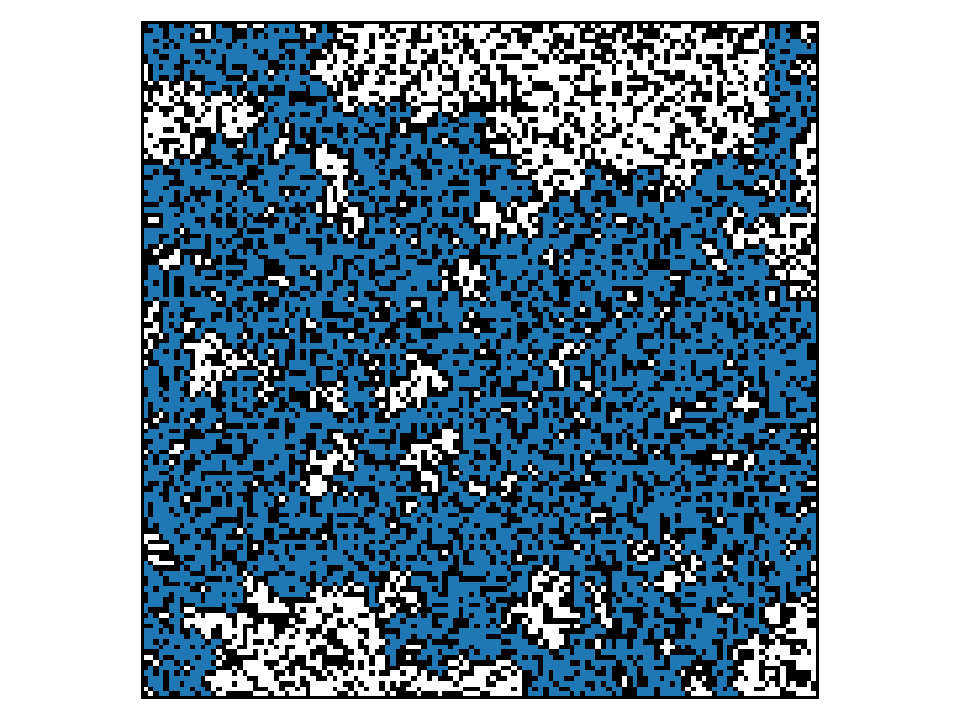
\includegraphics[width=1\linewidth]{malla.pdf}
    \caption{Malla de tamaño $128$ por $128$ para una probabilidad de ocupación de $0.6$ usando la semilla $15$. El negro indica sitios no ocupados, el blanco indica sitios ocupados que no pertenecen a un cluster percolante y el color indica el cluster percolante.}
    \label{fig:cluster}
\end{figure}

Con esta estructura base del código, se procedió a realizar simulaciones sistemáticas. Para cada combinación de los parámetros \( L \), \( p \) y nivel de optimización, el programa se ejecutó 10 veces utilizando diferentes semillas aleatorias. Se consideraron cinco tamaños de malla: \( L = 32, 64, 128, 256, 512 \); treinta valores de \( p \) distribuidos entre 0 y 1, con mayor densidad (10 valores) en la región crítica entre 0.55 y 0.65; y cinco niveles de optimización del compilador: \texttt{-O0}, \texttt{-O1}, \texttt{-O2}, \texttt{-O3} y \texttt{-Ofast}.

\subsection{Automatización con Makefile}

Para automatizar las distintas tareas del proyecto, se implementó un archivo \texttt{Makefile} con múltiples \textit{targets}, cada uno diseñado para realizar una tarea específica relacionada con la compilación, ejecución, análisis y validación del código. Los \textit{targets} que tienen \texttt{ARGS} frente al nombre reciben los valores de \texttt{L}, \texttt{p}, \texttt{seed} y \texttt{bool\_grafica} de la línea de comandos para realizar la tarea que ejecutan. Estos argumentos se deben pasar con la siguiente sintaxis:

\begin{center}
    \texttt{make nombre\_target ARGS="L p seed bool\_grafica"}
\end{center}


Por ejemplo, el siguiente comando ejecutaría y graficaría la malla de \texttt{L=512}, \texttt{p = 0.6}, \texttt{seed = 10} y \texttt{bool\_grafica = 1}:

\begin{center}
    \texttt{make simul ARGS="512 0.6 10 1"}
\end{center}

A continuación se describe la funcionalidad de cada uno de estos comandos:

\begin{itemize}
    \item \texttt{make analisis}: compila y ejecuta el código para todas las combinaciones de \( L \), \( p \) y niveles de optimización especificadas anteriormente, utilizando 50 semillas distintas. Los datos generados se procesan mediante un script en Python, que produce las gráficas en formato PDF presentadas en la sección de resultados.

    \item \texttt{make simul ARGS}: compila y ejecuta una simulación individual con los valores de \( L \), \( p \) y semilla aleatoria especificados. Posteriormente, genera una visualización del cluster percolante al pasar \texttt{bool\_grafica = 1}.
    
    \item \texttt{make test}: ejecuta pruebas unitarias utilizando la librería Catch2\cite{catch2} sobre cuatro casos base: una malla completamente vacía (\( p = 0 \)), una malla completamente ocupada (\( p = 1 \)), una malla con una línea horizontal de unos (para verificar percolación horizontal) y una con una línea vertical (para verificar percolación vertical). Estas pruebas comprueban la detección correcta de clusteres percolantes y el cálculo de sus tamaños.
    
    \item \texttt{make debug}: compila el programa con banderas de depuración y lo ejecuta bajo GDB\cite{GDB} para facilitar el análisis detallado de errores.
    
    \item \texttt{make valgrind ARGS}: compila el programa con banderas de depuración y ejecuta Valgrind\cite{Valgrind} para detectar pérdidas de memoria o accesos inválidos en un caso de prueba.
    
    \item \texttt{make profile ARGS}: genera informes de \textit{flat profiling} usando la herramienta \texttt{perf}\cite{perf} y \texttt{gprof}\cite{gprof}, tanto para la versión optimizada como para una versión previa no optimizada del código. Se le pueden pasar los argumentos para el caso de probabilidad crítica (\( L = 128 \), \( p = 0.59271 \)), sin embargo, el \textit{profiling} es más provechoso para tamaños de malla más grandes. Esta comparación se analiza en detalle en la sección de Dificultades y optimizaciones.
    
    \item \texttt{make coverage}: ejecuta los casos de prueba y genera un reporte en formato HTML que muestra la cobertura del código utilizando \texttt{gcovr}\cite{gcovr}.
    
    \item \texttt{make clean}: elimina archivos binarios, intermedios y temporales, incluyendo ejecutables, archivos \texttt{.gcda}, \texttt{.gcno}, \texttt{.txt}, \texttt{.pdf} y carpetas como \texttt{resultados} o \texttt{coverage}.

    \item \texttt{make report}: crea este informe a partir de un archivo latex y las figuras en fomato PDF en el repositorio.
    
\end{itemize}

\section{Resultados y análisis de resultados}

Una vez obtenidos todos los archivos \texttt{.txt} que almacenan en su primera columna los booleanos que determinan si existe un cluster percolante, en su segunda columna el tamaño del cluster percolante más grande, en su tercera columna el \textit{Wall time} y en su cuarta columna el \textit{CPU time}, para cada semilla manteniendo fijos los valores de tamaño de la malla y la probabilidad de ocupación, se realiza el procesamiento de los resultados obtenidos junto con sus correspondientes graficaciones mediante dos scripts de \textit{Python}, \texttt{clusters.py} y \texttt{probperc.py}.
\vspace{0.2 cm}

Por un lado \texttt{clusters.py} es el script encargado de realizar las graficaciones de la malla, detectando los estados no ocupados, los estados ocupados que no pertenecen a clusters percolantes y los estados que pertenecen a clusters percolantes. En la figura \ref{fig:cluster} se puede evidenciar un ejemplo de la graficación dada por \texttt{clusters.py}. Por el otro lado, el script \texttt{probperc.py} es el script encargado de hallar la probabilidad de cluster percolante, el promedio del tamaño de cluster percolante más grande y los tiempos computacionales. A continuación, se realiza una descripción de lo realizado y los resultados obtenidos.

\subsection{Probabilidad de percolación}

Para obtener la probabilidad de percolación en función de la probabilidad de ocupación para distintos valores del tamaño de la malla, para cada pareja $(L, p)$ se realizó un conteo de los casos para los cuales se obtuvo percolación, siendo que se trabajó con $50$ semillas para el generador aleatorio. En la figura \ref{fig: probabilidad} se evidencian los resultados obtenidos para la probabilidad de percolación.

\begin{figure}[H]
    \centering
    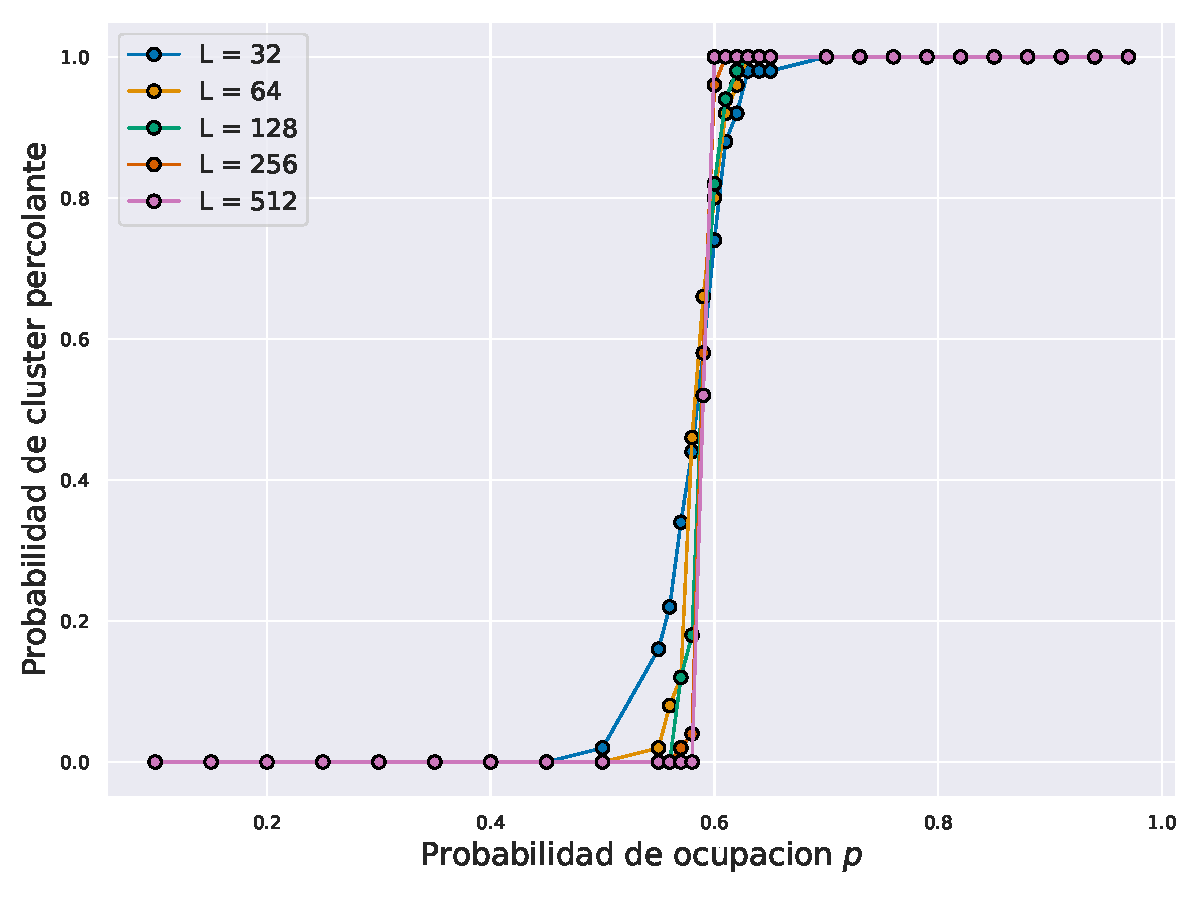
\includegraphics[width=1\linewidth]{Probabilidadcluster.pdf}
    \caption{Probabilidad de obtener cluster percolante en función de la probabilidad de ocupación $p$ para distintos tamaños de la malla. Se obtuvieron usando 50 semillas.}
    \label{fig: probabilidad}
\end{figure}

Nótese que conforme el tamaño de la malla aumenta, la probabilidad crítica de percolación $p_c$ tiende a su valor teórico, de modo que concuerda con lo esperado. Para el tamaño de malla $512$ por $512$ se obtuvo una probabilidad crítica de $p_c = 0.6$, puesto que a partir de este valor la probabilidad de obtener un cluster percolante siempre es $1$. El valor obtenido para la percolación crítica se encuentra sujeto a los intervalos de probabilidad de ocupación tomados en la región crítica, de forma que si se toman intervalos más pequeños para $p$ en la región crítica, se podría determinar con mejor precisión la probabilidad de percolación crítica asumiendo tamaños de malla más grandes.

\subsection{Tamaño promedio del cluster más grande}

Para determinar el tamaño del cluster percolante más grande para cada pareja de valores $(L, p)$, se realizó el promedio de los tamaños de cluster percolante más grande de las $50$ semillas usadas. Puesto que los valores registrados corresponden a promedios, a cada dato reportado se le asignó la desviación estándar de los $50$ tamaños para las diferentes semillas como medida del error del dato reportado. En la figura \ref{fig: tamano} se evidencian los resultados obtenidos para el tamaño promedio del cluster percolante más grande normalizado, es decir, se normaliza este valor respecto a su correspondiente valor de malla. Cabe recalcar que se omitieron los valores de probabilidad de ocupación para los cuales no se tienen clusters percolantes para ninguno de los tamaños de la malla.

\begin{figure}[H]
    \centering
    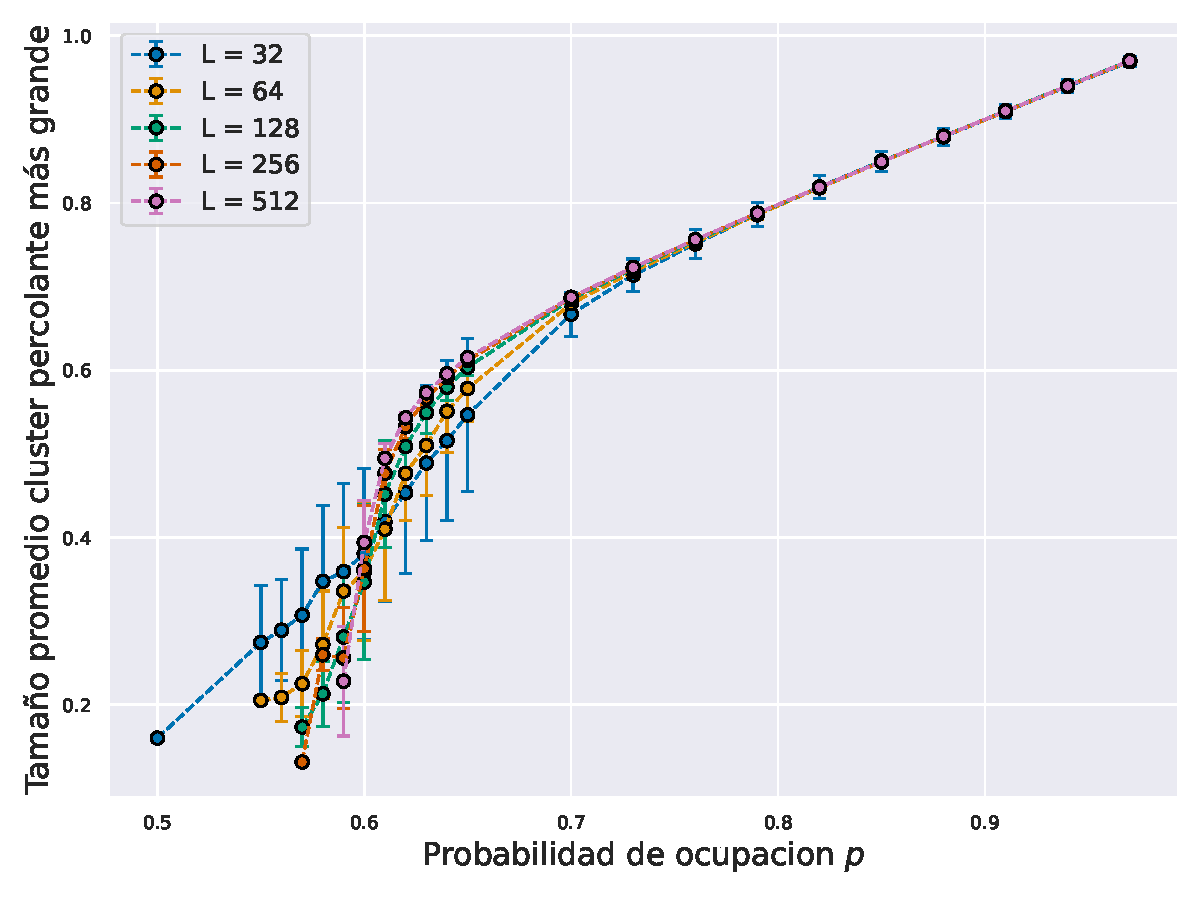
\includegraphics[width=1\linewidth]{Tamanocluster.pdf}
    \caption{Tamaño promedio del cluster percolante más grande relativo al tamaño de la malla correspondiente obtenido en función de la probabilidad de ocupación $p$ para distintos tamaños de la malla. Se obtuvieron usando 50 semillas.}
    \label{fig: tamano}
\end{figure}

Mediante los resultados obtenidos, se puede evidenciar que la proporción del cluster percolante más grande en promedio respecto al tamaño de la malla presenta un comportamiento de crecimiento conforme la probabilidad de ocupación aumenta, esto para todos los tamaños de malla. Para los primeros valores de $p$ a partir de los cuales se empezó a registrar percolación, se puede observar que dichos promedios presentan desviaciones estándar considerables, y conforme la probabilidad de ocupación es mayor, la desviación estándar de todos los datos reportados disminuye. Si bien los resultados de los diferentes tamaños de malla se encuentran más dispersos en la región crítica, una vez superada esta región todos los tamaños de cluster promedio más grande para todos los tamaños de malla convergen a una misma relación aproximadamente lineal. 

\subsection{Tiempo de cómputo para cada optimización}

En lo que respecta al tiempo de cómputo en función del tamaño de la malla para cada optimización, se decidió trabajar con el tiempo empleado en detectar clusters percolantes para todas las probabilidades de ocupación y semillas, manteniendo fijo el valor del tamaño de la malla y el optimizer empleado. Se registraron tanto el \textit{CPU time} como el \textit{Wall time} para cada pareja $(\mathrm{OPTIMIZER}, L)$. 
\vspace{0.2 cm}

En un principio se había optado por registrar un tiempo de cómputo total de lo que tardaba el código en detectar clusters percolantes para cada valor $(\mathrm{OPTIMIZER}, L, p)$ para todas las $50$ semillas. Una vez registrados estos tiempos, se promediaban todos aquellos que correspondiesen a un mismo optimizer y a un mismo tamaño de malla y se le asignaba la desviación estándar como medida de error del dato registrado, es decir, se retiraba la dependencia del parámetro $p$. Se optó por no tomar este camino en tanto que se evidenció que existía una relación entre la probabilidad de ocupación y los tiempos de cómputo, de forma que los diferentes datos para un mismo par $(\mathrm{OPTIMIZER}, L)$ pero diferentes $p$ se encontraban muy dispersos y los errores registrados eran relativamente grandes. Esta dependencia entre la probabilidad de ocupación y los tiempos de cómputo se debe a que entre mayor sea la cantidad de estados ocupados, el código debe realizar una mayor cantidad de iteraciones para determinar si pertenece o no a un cluster percolante.
\vspace{0.2 cm}

En la figura \ref{fig: tiempos} se reportan los tiempos computacionales de \textit{CPU time} y \textit{Wall time} para los distintos valores del tamaño de la malla y los diferentes optimizers. Cabe recalcar que en vista de que los tiempos computacionales registrados no surgen a partir de un análisis estadístico de promedios y desviaciones estándar, no se reportaron errores de estos datos de esta índole. En su lugar, los errores de los tiempos registrados corresponden a los errores de medición intrínsecos de las librerías de C++ empleadas para medir el tiempo, \textit{Chrono} y \textit{ctime}.

\begin{figure}[H]
    \centering
    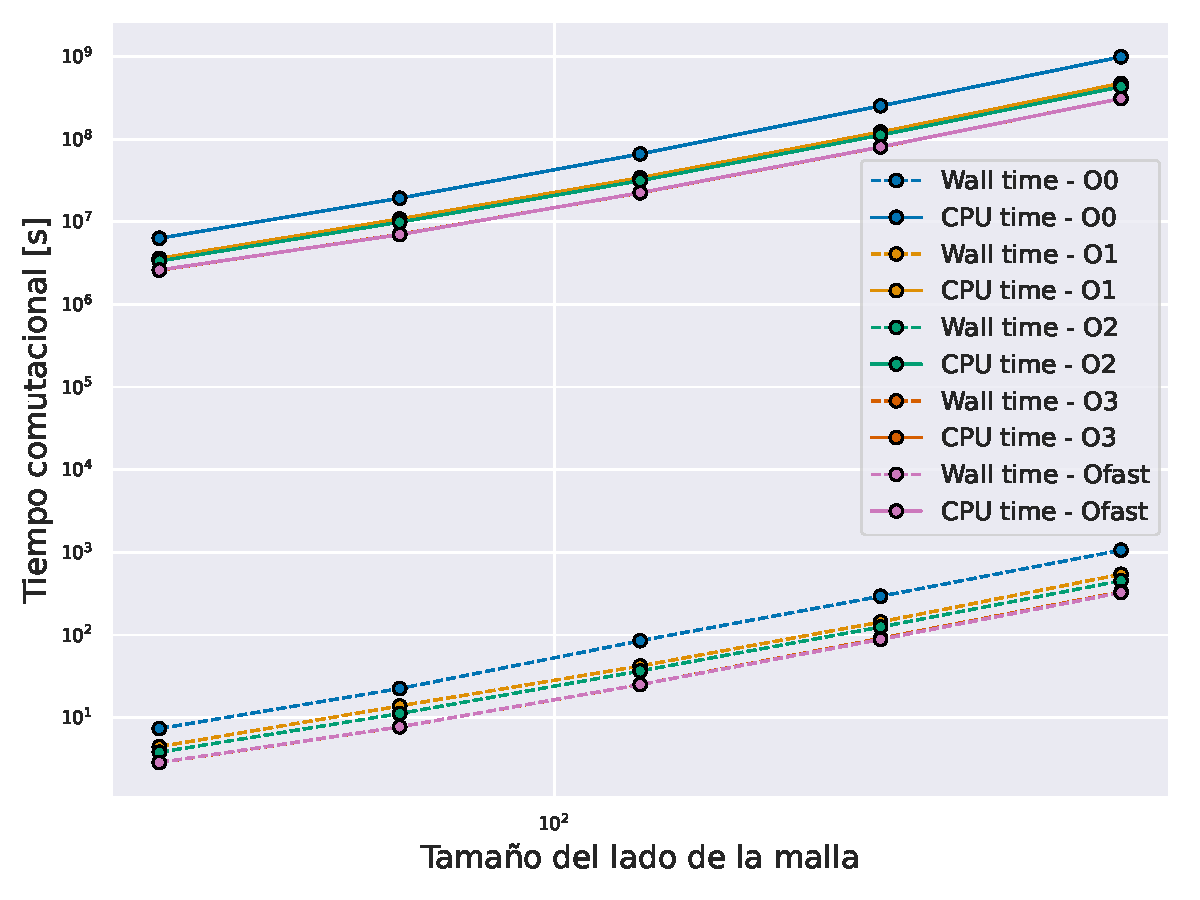
\includegraphics[width=1\linewidth]{Tiempos.pdf}
    \caption{Tiempos computacionales obtenidos (CPU time \& Wall time) para determinar percolación para $5$ tamaños de malla, $30$ probabilidades de ocupación y $50$ semillas (todas las combinaciones de estos tres parámetros) para los diferentes optimizers en función del tamaño de la malla. Gráfica en escala log-log.}
    \label{fig: tiempos}
\end{figure}

El comportamiento de los tiempos computacionales con respecto a los tamaños de la malla es el esperado, pues nótese que se presenta un comportamiento lineal de cada curva en escala log-log, de forma que esto refleja un comportamiento exponencial tal que el tiempo computacional crece rápidamente. Se observa que el optimizador \texttt{-O0} tiene los tiempos más altos tanto en \textit{Wall} como en \textit{CPU time}. Por otro lado, los optimizadores \texttt{-O1}, \texttt{-O2}, \texttt{-O3} y \texttt{-Ofast} mejoran progresivamente el rendimiento del código, siendo que \texttt{-Ofast} presenta el mejor desempeño; sin embargo, la diferencia con \texttt{-O3} es pequeña, lo que indica que estas optimizaciones tienen un gran efecto en el rendimiento del programa, pero que presentan ganancias marginales a partir de cierto punto.

\subsection{Flat Profile para la probabilidad crítica $p_c$}

Como fue descrito en la \textbf{ Sección A (Código base)}, en el archivo \texttt{functions.cpp} se implementan las herramientas básicas para identificar y etiquetar los clusteres, únicamente recorriendo los sitios ocupados en la primera fila y la primera columna de la malla de tamaño LxL. En la versión inicial de la misma, en el archivo \texttt{functions\_viejo.cpp}, se aplicaban las mismas funciones con la diferencia de que esta exploraba toda la superficie de la malla LxL. 

Así pues, en la implementación inicial, la función \texttt{hay\_cluster\_percolante.cpp} concentra el $53.5\%$ de los ciclos de CPU, seguida por \texttt{generar\_malla\_1D.cpp} que acapara un $28.8\%$. Al comparar estos resultados con la implementación final, se obtiene que \texttt{generar\_malla\_1D.cpp} concentra el $49.3\%$ de los ciclos, mientras que \texttt{hay\_cluster\_percolante.cpp} baja a un $20.3\%$. 

Se observa una inversión en la carga de cómputo entre ambas versiones. Cuando se amplía la zona de la malla explorada, el número de llamados a \texttt{dfs()} crece, generando invocaciones redundantes que sobrecargan el análisis sin aportar al objetivo principal.

\subsection{Dificultades y optimizaciones}

Una de las principales dificultades encontradas durante el desarrollo del proyecto fue la implementación inicial de la función \texttt{dfs()}, la cual realizaba llamadas recursivas para explorar los vecinos de un sitio ocupado. Esta aproximación recursiva generaba un desbordamiento de pila (\textit{stack overflow}) en mallas grandes, como aquellas con \( L = 512 \), impidiendo que se completara la detección de clusteres percolantes y el cálculo de su tamaño.

La solución consistió en reemplazar la recursividad por una implementación iterativa utilizando un objeto \texttt{stack} de la biblioteca estándar \texttt{<stack>}. Esta estructura permitió gestionar explícitamente el recorrido por vecinos: se elimina el sitio actual de la pila y se agregan únicamente los vecinos ocupados y no etiquetados. Cuando la pila se vacía, se retorna el tamaño del cluster. Esta versión iterativa evita el desbordamiento y mejora el control del flujo de ejecución. La lógica completa está documentada mediante comentarios en \texttt{functions.cpp}.

Una vez resuelto este problema, se identificó una segunda optimización importante. La versión original de \texttt{hay\_cluster\_percolante()} evaluaba la conectividad para toda la malla (\( L \times L \)), lo cual era innecesariamente costoso para el objetivo de detectar si existe al menos un cluster percolante. Se observó que basta con explorar únicamente los sitios ocupados en la primera fila y la primera columna, ya que cualquier cluster percolante debe estar conectado a uno de estos bordes. Esta optimización redujo significativamente el tiempo de ejecución.

La mejora lograda puede observarse en los reportes de \textit{profiling} obtenidos con \texttt{perf} discutidos anteriormente, comparando dos versiones del código: una optimizada que solo recorre la primera fila y columna (\texttt{functions.cpp}), y otra sin optimización que recorre toda la malla (\texttt{functions\_viejo.cpp}). El caso analizado corresponde a los parámetros \( L = 128 \), \( p = 0.59271 \) y \texttt{seed} = 10.


\section{Conclusiones}

Se verificó numéricamente la existencia de una transición de fase en la percolación, tal que la probabilidad de aparición de un cluster percolante tiende a una función escalón conforme aumenta el tamaño de la malla, con un valor crítico de $p_c = 0.6$ para $L = 512$, valor cercano a la probabilidad crítica de ocupación teórico $p_c \approx 0.59271$. En cuanto al tamaño promedio del cluster percolante más grande, se evidencia que este es más grande conforme aumenta $p$, convergiendo para todos los tamaños de malla a una misma relación lineal para $p > p_c$, con menor dispersión en esta región.
\vspace{0.2 cm}

La comparación entre diferentes niveles de optimización evidencia que \texttt{-O3} y \texttt{-Ofast} logran reducir el tiempo computacional de forma considerable frente a los otros niveles de optimización, de forma que se confirma la importancia de las optimizaciones de compilación en simulaciones que escalen de forma exponencial. No solo los niveles de optimización del compilador influyeron en la reducción en el tiempo de cómputo, sino que a nivel algorítmico, reemplazar la versión recursiva de \texttt{dfs()} por una versión iterativa evitó errores en el desbordamiento de pila para mallas grandes con altas probabilidades de ocupación. Asimismo, limitar el análisis a la primera fila y la primera columna resultó en una mejora en la eficiencia en cuanto a que se busca determinar únicamente los clusters percolantes, no se requiere detectar y etiquetar el resto de clusters.
\vspace{0.2 cm}

Por otro lado, el uso de herramientas como \textit{Makefile}, \textit{Valgrind}, \textit{gprof}, \textit{perf} y \textit{gcovr} permitieron un desarrollo reproducible, depurable y evaluable del trabajo.
\vspace{0.2 cm}

\bibliography{report}


\section{Anexos}

\subsection{Repositorio GitHub}

En el siguiente repositorio de GitHub se encuentran los códigos empleados en C++, Python, el \textit{Makefile}, los archivos \texttt{.pdf} donde se encuentran tanto las figuras como este reporte: \url{https://github.com/JuanSeguraUNAL/Percolacion-malla-bidimensional}.

\subsection{Herramienta trabajo grupal: Todoist}

Para la coordinación del trabajo y la asignación de tareas y pendientes se trabajó con Todoist, tal que se cuadraron fechas para reuniones digitales y las fechas para cada uno de los pendientes.

\begin{figure}[H]
    \centering
    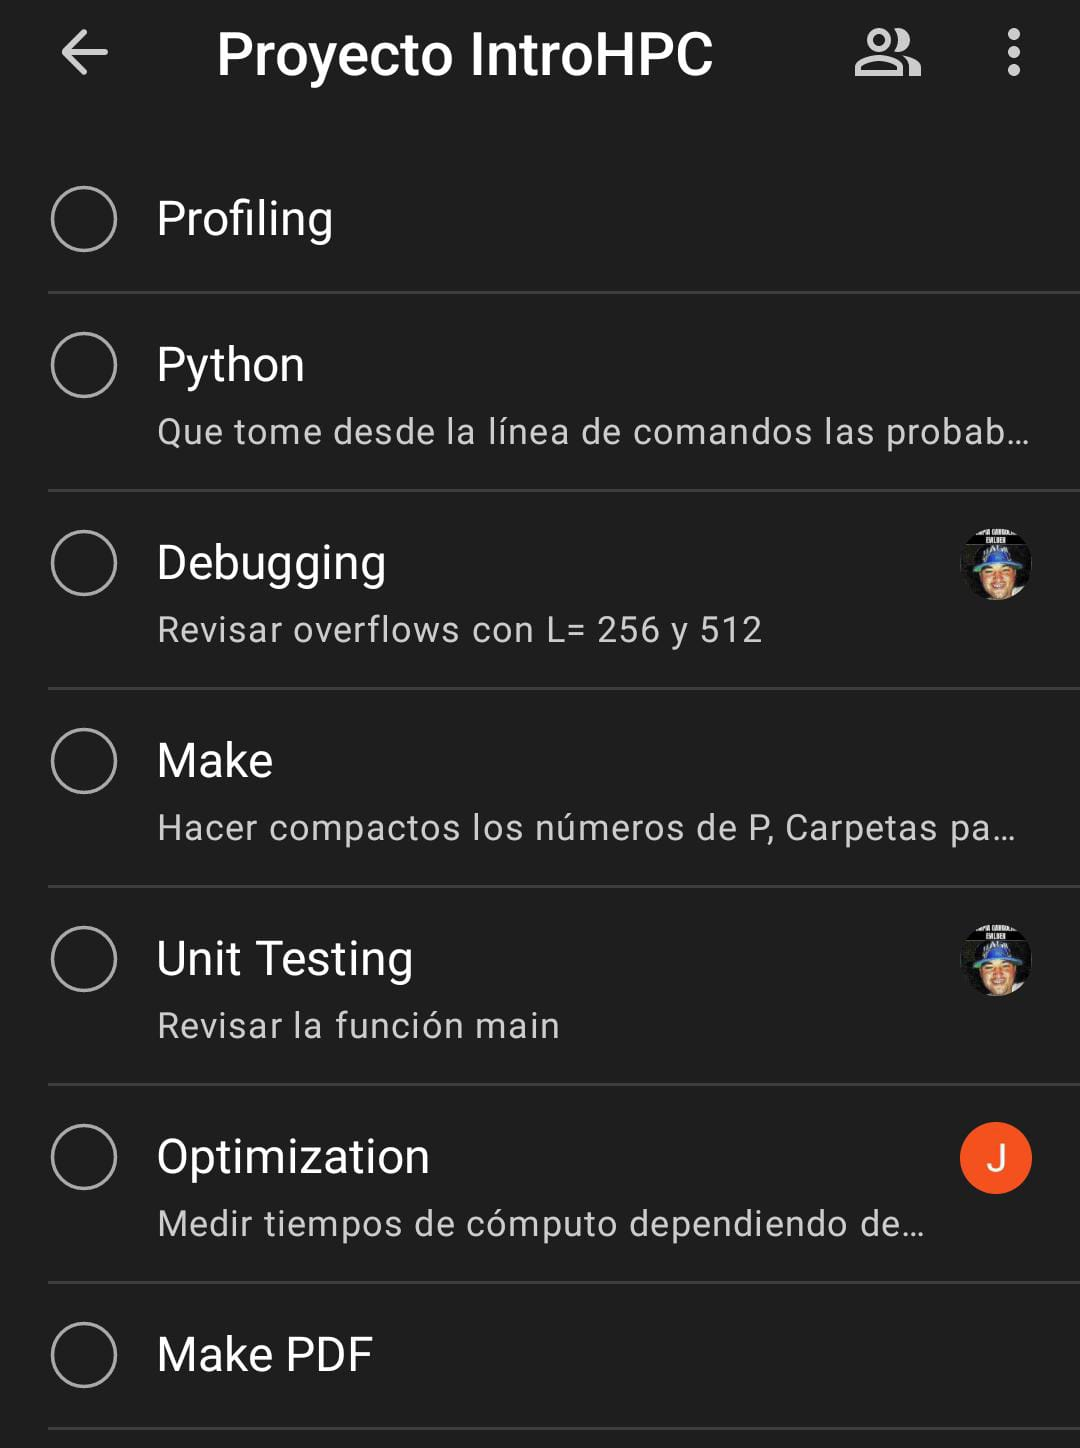
\includegraphics[width=0.8\linewidth]{todoist.jpeg}
    \caption{Asignación de tareas en Todoist.}
    \label{fig: todoist}
\end{figure}


\end{document}
%
% ****** End of file apssamp.tex ******